\begin{figure*}[htb]
    \centering
    \subfloat[Accury \textit{w.r.t.} Ratio of Unknown Samples]{
        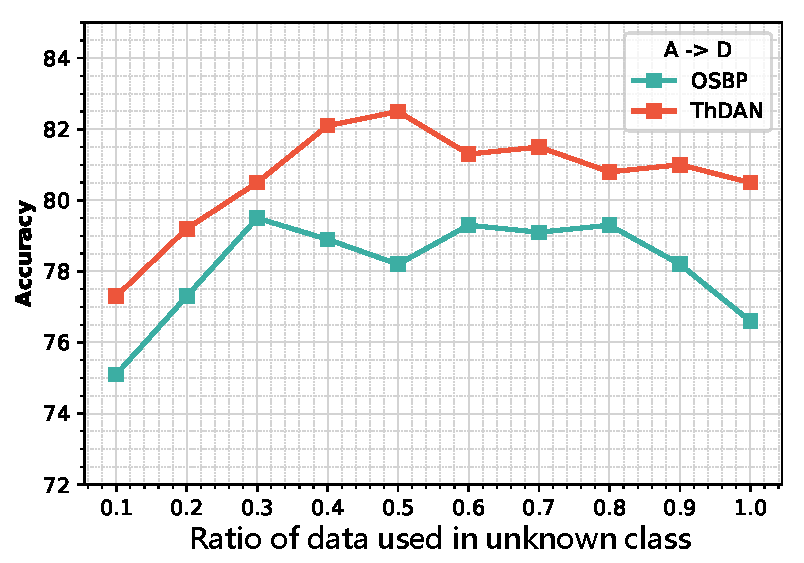
\includegraphics[width=0.34\textwidth]{contents/figures/pdf/analysis/nuknown_change.pdf} 
        \label{figure: ration of unknown f}
    } 
    \subfloat[Accury \textit{w.r.t.} Number of Unknown Classes]{
        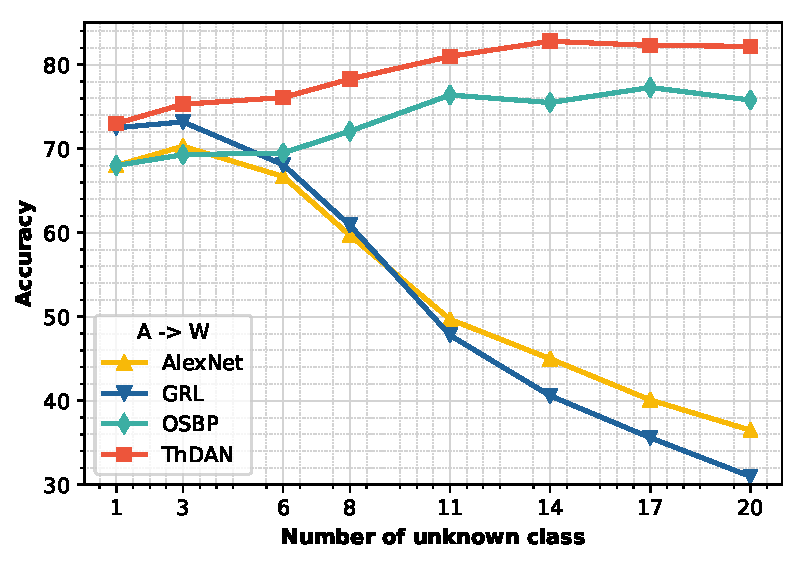
\includegraphics[width=0.33\textwidth]{contents/figures/pdf/analysis/class_change.pdf} 
        \label{figure: number of unknown class f}
    }
    \\
    \caption{
        (\textbf{a}): 
        The prediction accuracy of our method when we changed the ratio of unknown samples in the adaptation task \textit{A$\to$D}. 
        (\textbf{b}): 
        The prediction accuracy of our method when we changed the number of unknown classes in the adaptation task \textit{A$\to$W}. 
    }
    \label{figure: analysis}
\end{figure*}